\documentclass[12pt]{article}
\usepackage[utf8]{inputenc}
\usepackage{indentfirst}
\usepackage{graphicx}
\usepackage{hyperref}
\hypersetup{
    colorlinks,
    citecolor=black,
    filecolor=black,
    linkcolor=red,
    urlcolor=blue,
}

\title{\textbf{Data Wrangling Report}}
\author{Octave Cinquanta}
\date{October 2021}

\begin{document}

\maketitle
\tableofcontents

\section{Introduction}

For the course of data wrangling, we were instructed with the recovery of a large set of data from theses.fr, a website collecting various information on theses such as their authors, their defense date, their abstract and the theses themselves. After successfully obtaining the required data-set, we were to be confronted by the issue of missing data, and find a way to deal with this problem. The next step was to investigate the common issues found within the data-set and try to understand them. Next was to find the different outliers hidden inside the data-set. Finally, we had to treat our data in order to obtain some preliminary results.

\section{Data Scraping}

The first task that was given to us was to create a scraping algorithm to collect data from these.fr.. The algorithm was to explore to website in search of links to multiple theses, and afterwards use these links to create a list of thesis authors registered on the website. The scraping algorithm used was programmed in python, and is included as well as commented in the Code Section of the report.

\section{Dealing with Missing Data}

\begin{figure}[h]
    \centering
    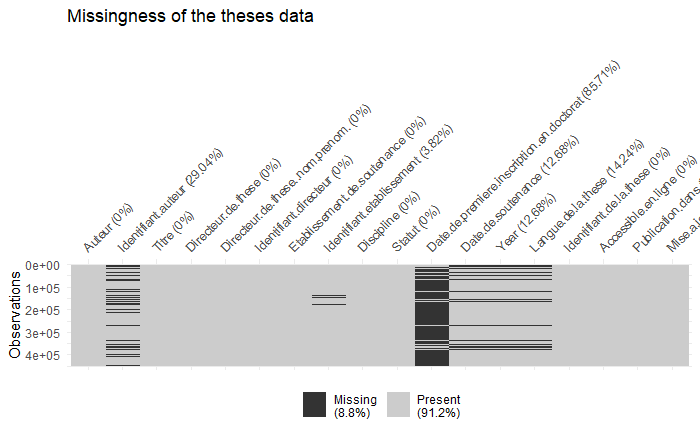
\includegraphics[width=\textwidth]{plot.png}
    \label{plot}
\end{figure}

The next task was to estimate the amount of missing data in our data-set and deal with this issue. We started by creating a \hyperref[plot]{plot} of the missing data that represents it as various bars corresponding to the different variables inside the data-set, as well as a table that resumes the percentage of missing data per column. On the following page is the mentioned table.

\begin{table}[ht]
\centering
\begin{tabular}{rrr}
  \hline
 & missing & \% \\ 
  \hline
Date.de.premiere.inscription.en.doctorat & 383668.00 & 86.00 \\ 
  Identifiant.auteur & 129989.00 & 29.00 \\ 
  Langue.de.la.these & 63765.00 & 14.00 \\ 
  Date.de.soutenance & 56746.00 & 13.00 \\ 
  Year & 56746.00 & 13.00 \\ 
  Identifiant.etablissement & 17085.00 & 4.00 \\ 
  Mise.a.jour.dans.theses.fr & 177.00 & 0.00 \\ 
  Directeur.de.these & 17.00 & 0.00 \\ 
  Directeur.de.these..nom.prenom. & 17.00 & 0.00 \\ 
  Titre & 9.00 & 0.00 \\ 
  Discipline & 5.00 & 0.00 \\ 
  Etablissement.de.soutenance & 4.00 & 0.00 \\ 
  Auteur & 2.00 & 0.00 \\ 
  Identifiant.directeur & 0.00 & 0.00 \\ 
  Statut & 0.00 & 0.00 \\ 
  Identifiant.de.la.these & 0.00 & 0.00 \\ 
  Accessible.en.ligne & 0.00 & 0.00 \\ 
  Publication.dans.theses.fr & 0.00 & 0.00 \\ 
   \hline
\end{tabular}
\end{table}

We can see that most columns do not contain missing data, or a rather small amount, but a few columns possess a significant amount of missing data. We can also notice that this missing data is not random for four columns: "Date.de.premiere.inscription.en.doctorat", "Date.de.soutenance", "Year" and "Langue.de.la.these". Those four columns are correlated as such: it looks as if a value is present in the first, then it is missing in the other three columns. We can make a hypothesis on why this is the case. It is likely that at the time of the registration of the thesis on the website, when it starts being written, that start date is registered in the first column but it is erased when that thesis is finished, and thus defended. As such as soon as that date disappears, the defense date is registered in its appropriate column. The year of the defense date obviously follows suit. As for the language, it is not a perfect correlation but it still is quite meaningful, likely because a thesis' languages are registered by the website once this thesis is completely written and defended. \\
The "number of pages" missing data imputation is included in the Code Section of the report.

\section{Investigating Common Issues}

Our third task was to investigate common issues found within the data-set. The first of these issues was the case of the first of January. Indeed, we computed that more than 62\% of theses were defended on a first of January, which is an obvious indication that there is an issue here with our data-set. We then decided to look into this problem by plotting the amount of theses defended on the first of January throughout the years.

\begin{figure}[h]
    \centering
    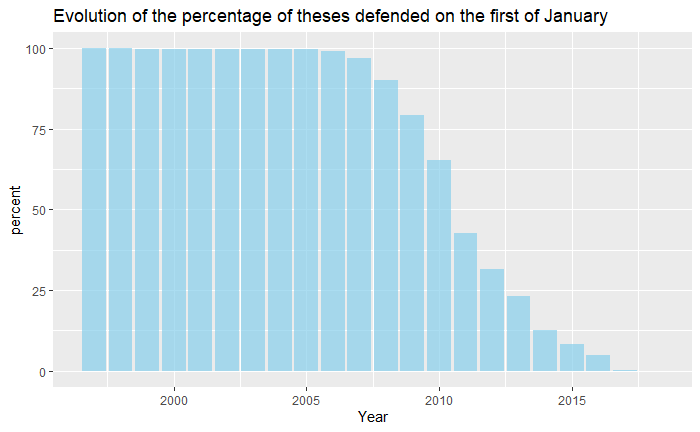
\includegraphics[width=\textwidth]{plot2.png}
    \label{plot2}
\end{figure}

As we can see on this \hyperref[plot2]{plot}, the percentage of theses defended on the first of January is overwhelming in the earliest years and through time gets smaller only to end up almost nonexistent by 2017. This can be explained by the fact that the website opened in 2011, and that it is most likely that many of the defense dates from earlier theses were lost, and that the missing data was then replaced with the first of January of the corresponding year, this would also explain the later years as it is almost impossible to defend a thesis on the first of January. \\
The next common issue to tackle was the case of homonyms. We calculated that the percentage of authors who had other authors as homonyms was slightly more than 2\%, which, on a data-set of this size, is not that rare. We also investigated the case of Cecile Martin, a person who defended 4 theses in 1991, 1994, 2000 and 2001. Such a feat is of course impossible, as such we lay the hypothesis that since these are all old theses, it is a possibility that when creating the data-set the same ID was assigned to 4 different Cecile based on their name, without checking first whether it could have been the same Cecile or not. \\
We also investigated the fact that more than 6\% of director IDs have commas in them, probably an imputing mistake made by the website. There is also a sudden drop of thesis defended in 2019 and 2020. It could be explained by the appearance of the Covid-19 pandemic, that had a major impact on all humanity at that time. The sickness itself probably prevented a number of students from defending their thesis at this time, maybe it was the lockdown that made it impossible to physically defend a thesis, or maybe it was that the theses jury itself was affected, or maybe even it was out of choice to choose to report the thesis defense, amongst many possibilities.

\section{Finding Outliers}

In this section, we looked at the supervisors who directed a large number of theses. Those numbers are such that they belong either to an homonym or a mistake, or to someone who dedicated his whole life to directing theses. One way to check whether this is the former or the latter would be to perform an internet search using a sort of scraper to find a Wikipedia page or another source of information confirming the direction of multiple theses using only the director's name. 

\section{Obtaining Preliminary Results}

In this final part, our job was to use the data-set to analyse certain data in interesting ways. The first analysis was of the evolution of the languages used in the writing of theses. We produced two graphs using both \hyperref[plot3]{ggplot} and \hyperref[plot4]{plotly} to represent this analysis. As we can see in these two graphs, the number of French theses is rather consistent throughout the years, but the number of English, bilingual and other languages is ever-increasing, especially in the more recent years, and especially English theses.

\begin{figure}[h]
    \centering
    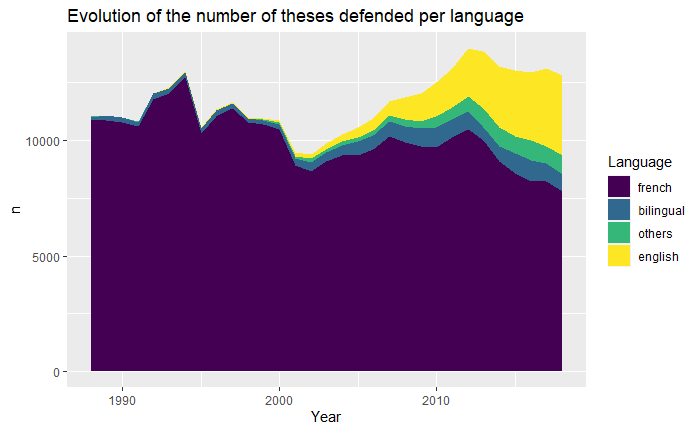
\includegraphics[width=\textwidth]{plot3.png}
    \label{plot3}
\end{figure}

\begin{figure}[h]
    \centering
    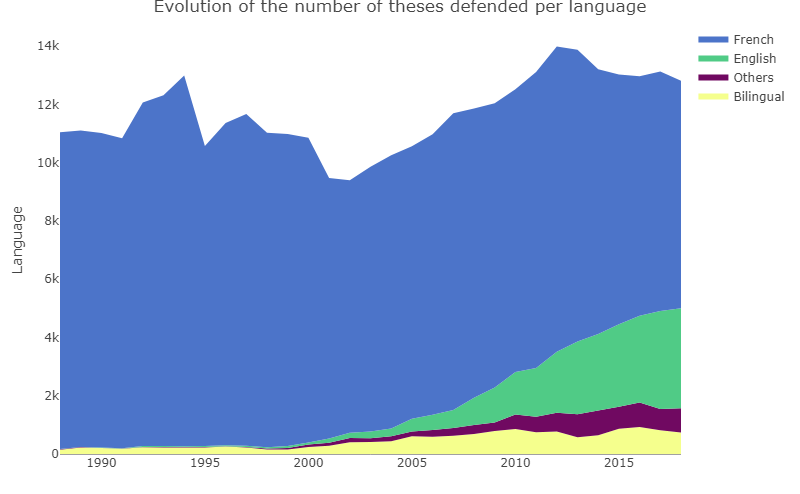
\includegraphics[width=\textwidth]{plot4.png}
    \label{plot4}
\end{figure}

The second analysis we had to do was to plot the re-partition of theses defended throughout the months. We can see on this \hyperref[plot5]{graph} that people have a tendency to defend in December, coinciding with the end of the calendar year. There is also a slight tendency in June, before the holidays and the summer in general, also coinciding with the end of the scholar year.

\begin{figure}[h]
    \centering
    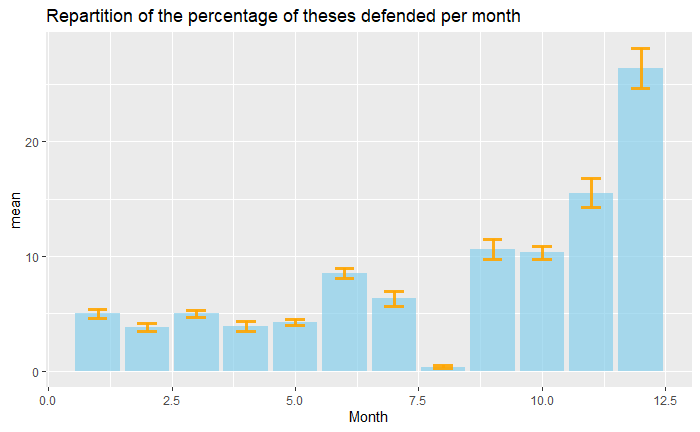
\includegraphics[width=\textwidth]{plot5.png}
    \label{plot5}
\end{figure}

\end{document}
